
%\section{Datasets}

The example analysis studied here involves a so-called Daltiz-plot analysis.  In such analyses, the distribution of events in a 2-D space is typically fit to extract some information of physical interest.  The regions of the Daltiz-plot that tend to have the highest sensitivity to the desired information are the {\em edges}.  Unfortunately, the edge regions also typically have the most background contamination and the least discrimination against background.  Therefore, traditional classifier-based selections tend to produce selections for Dalitz-plot analyses with lower efficiency near the edges.   

This study uses simulated event samples produced using the official LHCb simulation framework.
The software used for the generation of the events is described in LHCb publications as follows :

\begin{quote}
In the simulation, $pp$ collisions are generated using
PYTHIA~\cite{Sjostrand:2006za} 
with a specific LHCb configuration~\cite{LHCb-PROC-2010-056}.  Decays of hadronic particles
are described by EvtGen~\cite{Lange:2001uf}, in which final state
radiation is generated using PHOTOS~\cite{Golonka:2005pn}. The
interaction of the generated particles with the detector and its
response are implemented using the GEANT
toolkit~\cite{Allison:2006ve, Agostinelli:2002hh} as described in
Ref.~\cite{LHCb-PROC-2011-006}.
\end{quote}

All simulated event samples are generated inside the LHCb detector acceptance.
The signal used in this analysis consists of $D_s^\pm\to\pi^+\pi^-\pi^\pm$ decays, simulated
using the $\textrm{D}\_\textrm{DALITZ}$ model of EvtGen to simulate the intermediate resonances which contribute to the
three pion final state. The background candidates are three pion combinations reconstructed in
simulated samples of $c\bar{c}$ and $b\bar{b}$ events, where the charm and bottom quark decays are
inclusively modelled by EvtGen. The simulated events contain ``truth'' information which identifies them as
signal or background, and which identifies the physical origin of the three pion combinations reconstructed
in the $c\bar{c}$ and $b\bar{b}$ simulated samples.

\begin{figure}[] 
  \centering 
  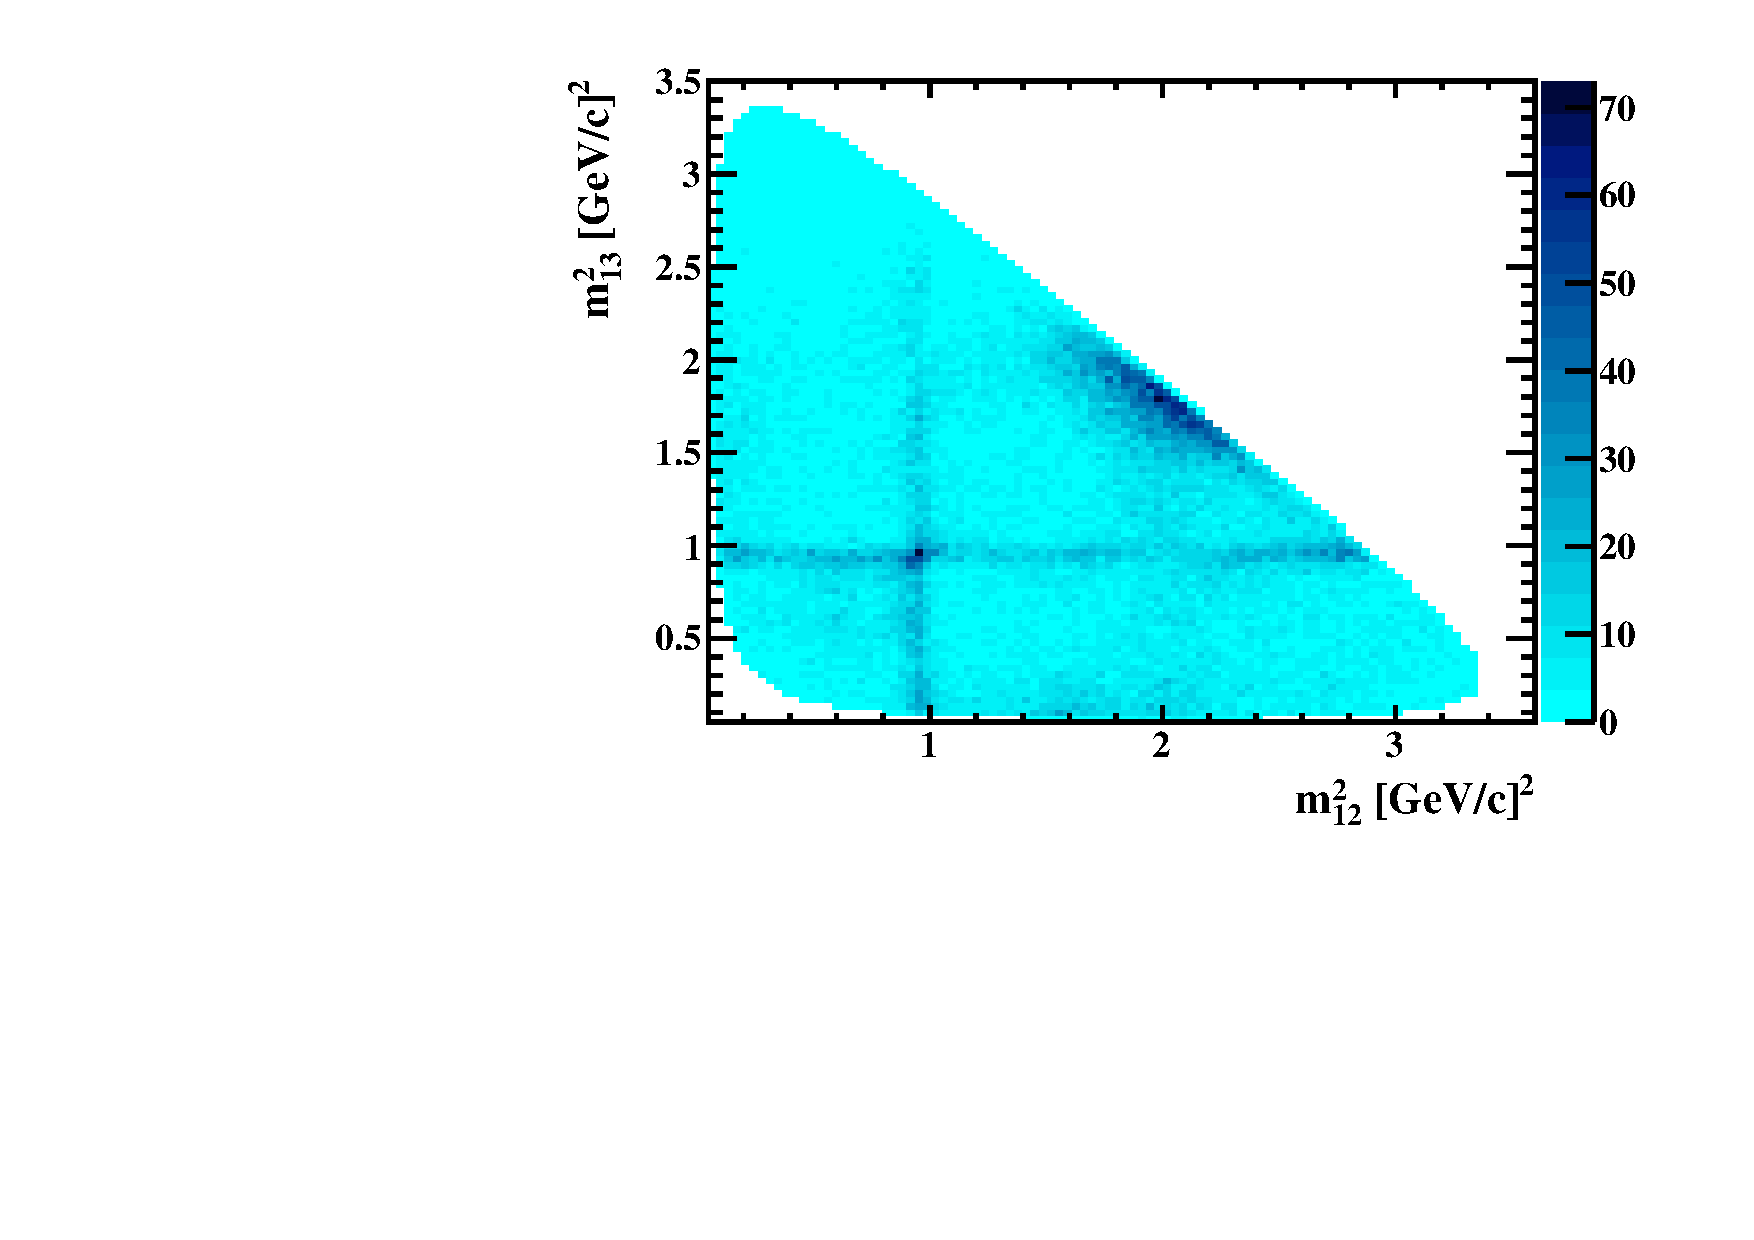
\includegraphics[width=0.49\textwidth]{DP_sig.pdf}
  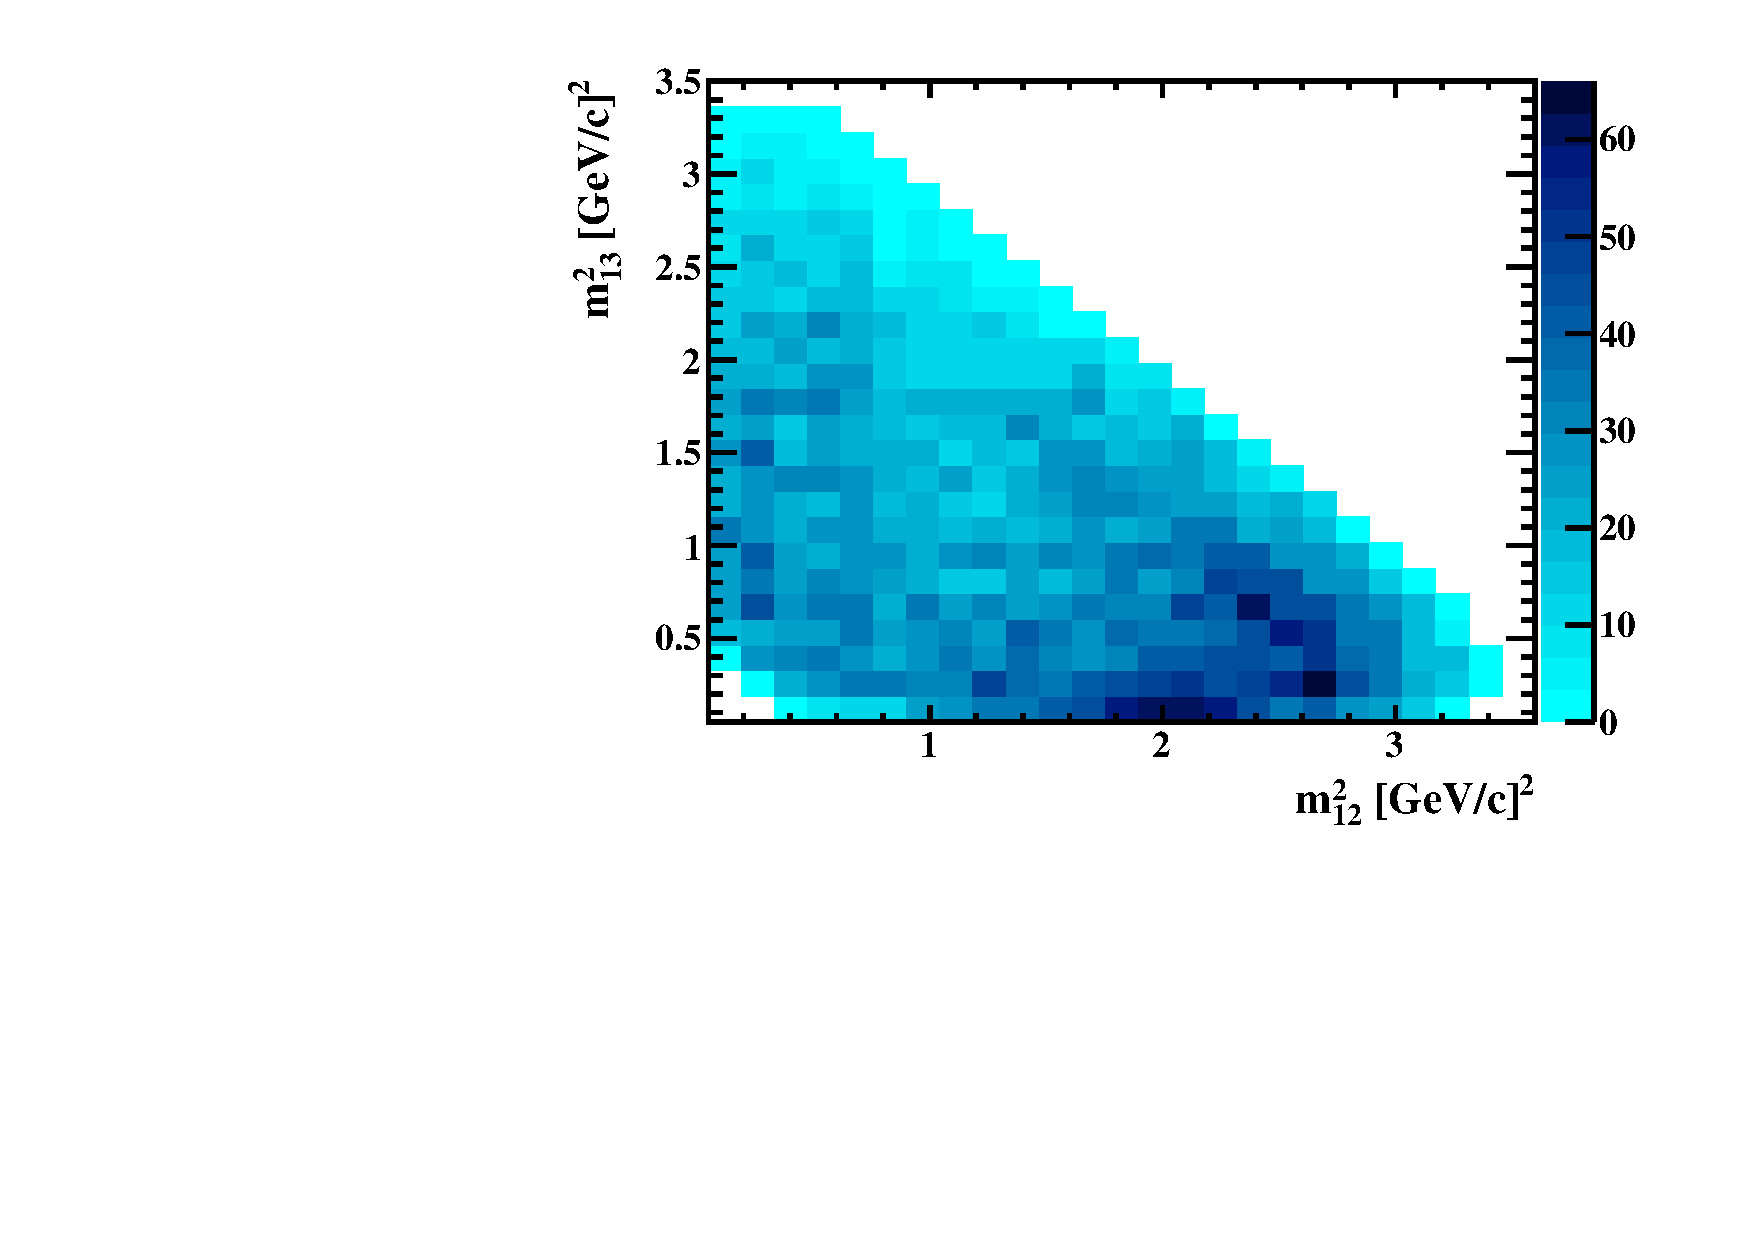
\includegraphics[width=0.49\textwidth]{DP_bkgd.pdf}
  \caption{\label{fig:dalitz} Dalitz-plot distributions for (left) signal and (right) background for the $D_s^\pm\to\pi^+\pi^-\pi^\pm$.  The three pions are labeled here as 1, 2 and 3.}
\end{figure}

Figure~\ref{fig:dalitz} shows the Dalitz-plot distributions for signal and background events.  These samples are split into training and testing samples and then various BDTs are trained.  Figure~\ref{fig:dalitz_results} shows the efficiency obtained for each classifier {\em vs} distance from the a corner of the Dalitz-plot.  The AdaBoost algorithm, as expected, produces a much lower efficiency in the interesting corner regions.  The kNNAdaBoost algorithm does not improve upon the AdaBoost result much.  This is likely due to the fact that while kNNAdaBoost uses non-local kNN information, it does not utilize global information.
The UGBFL (binned and unbinned kNN) and uBoost algorithms each produce an efficiency which is statistically consistent with uniform across the Dalitz plot.  


\begin{figure}[] 
  \centering 
  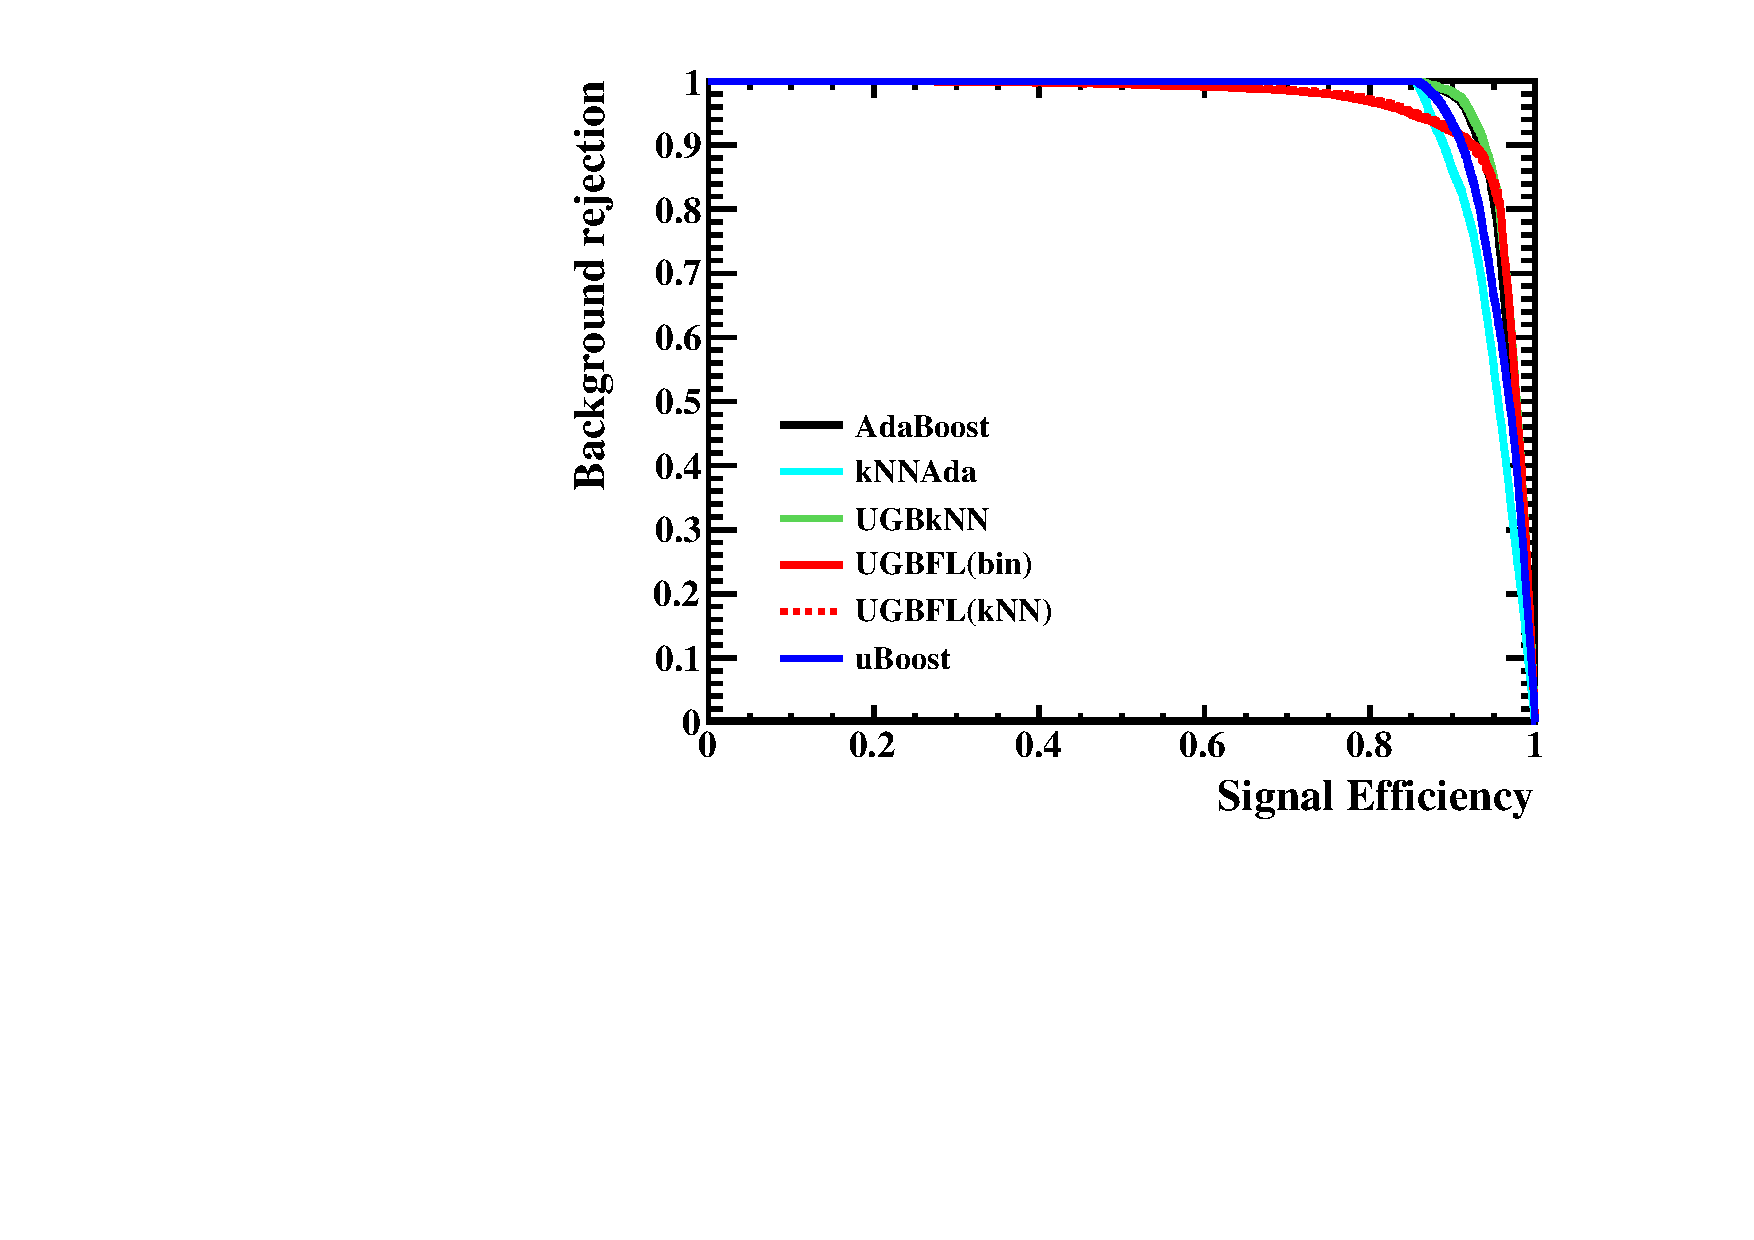
\includegraphics[width=0.49\textwidth]{ROC_DP.pdf}
  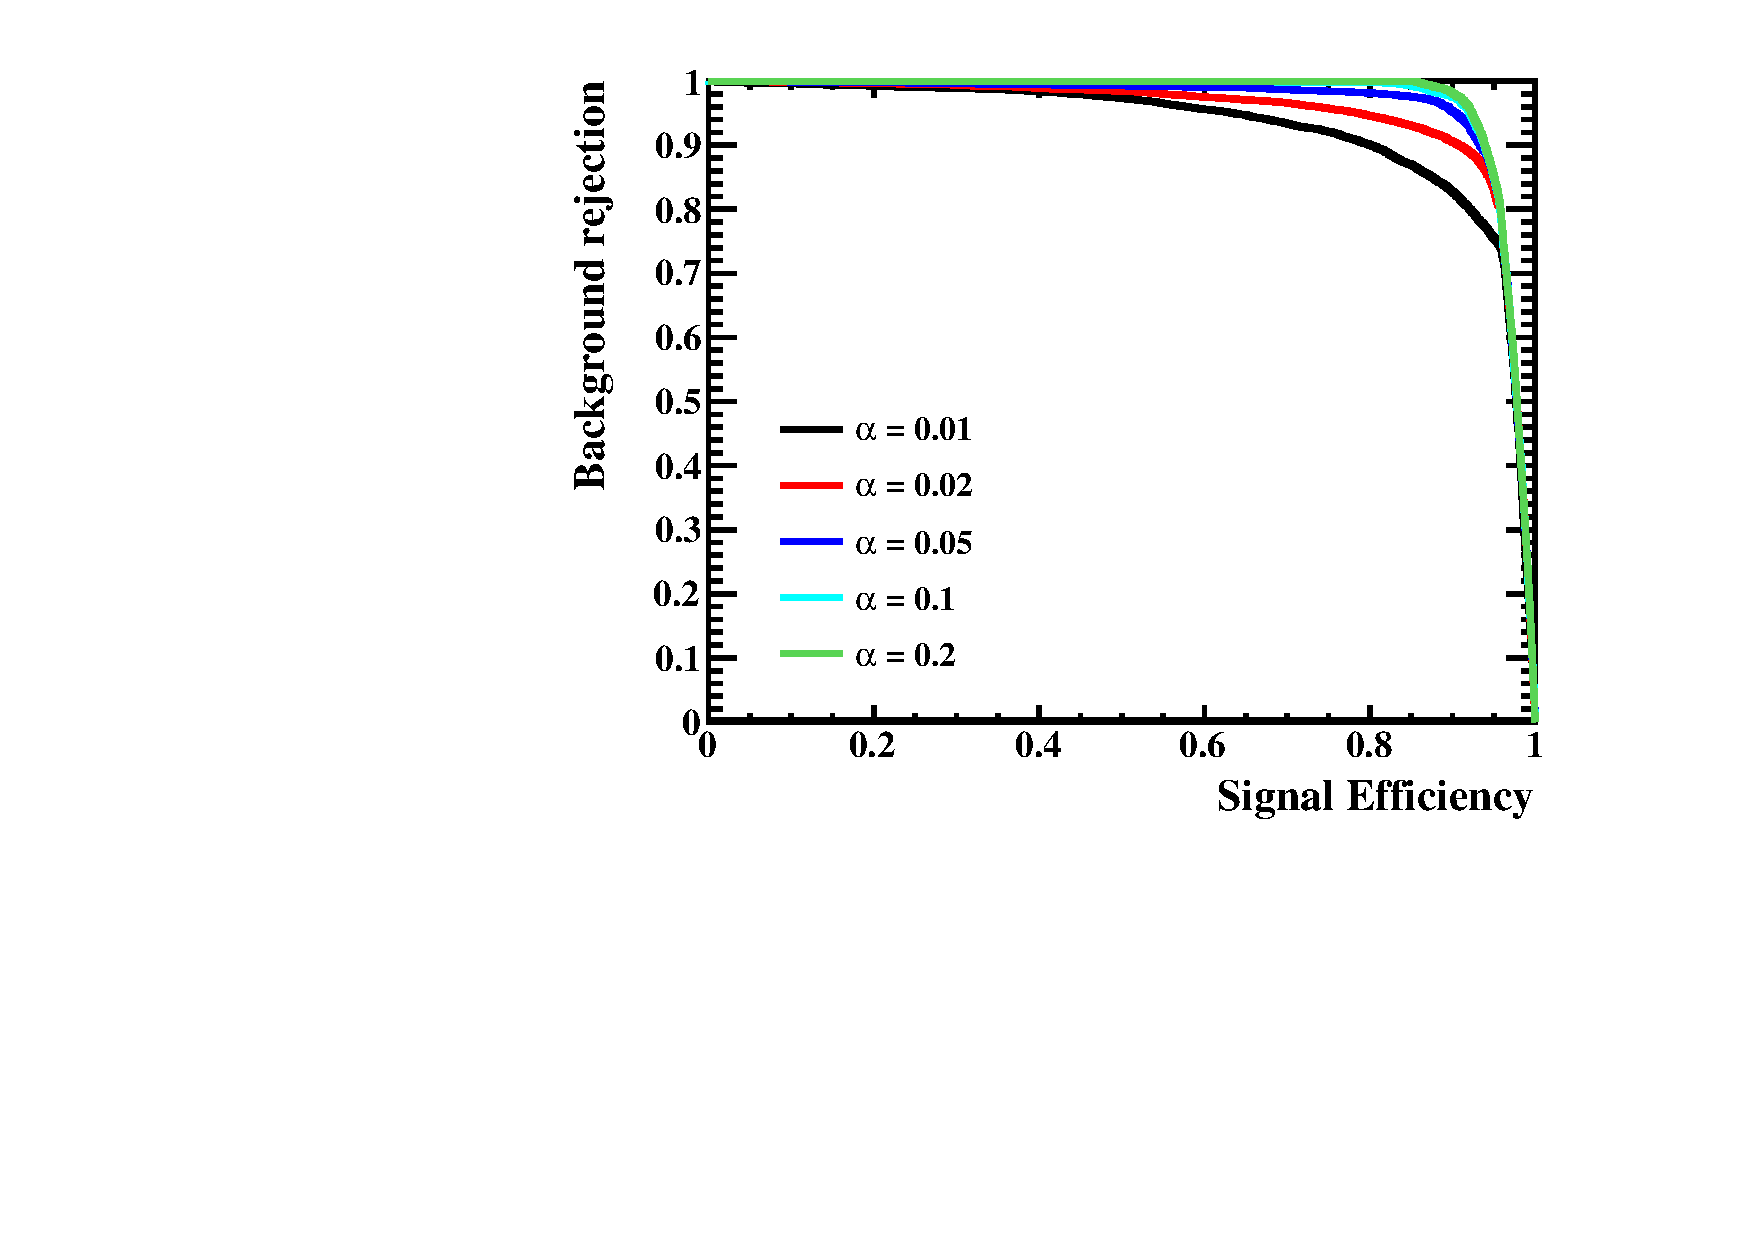
\includegraphics[width=0.49\textwidth]{ROC_DP_Alpha.pdf}
  \caption{\label{fig:dalitz_rocs} Efficiency {\em vs} distance to a corner of the Dalitz-plot.  An arbitrary working point of 50\% integrated efficiency is displayed.}
\end{figure}

\begin{figure}[] 
  \centering 
  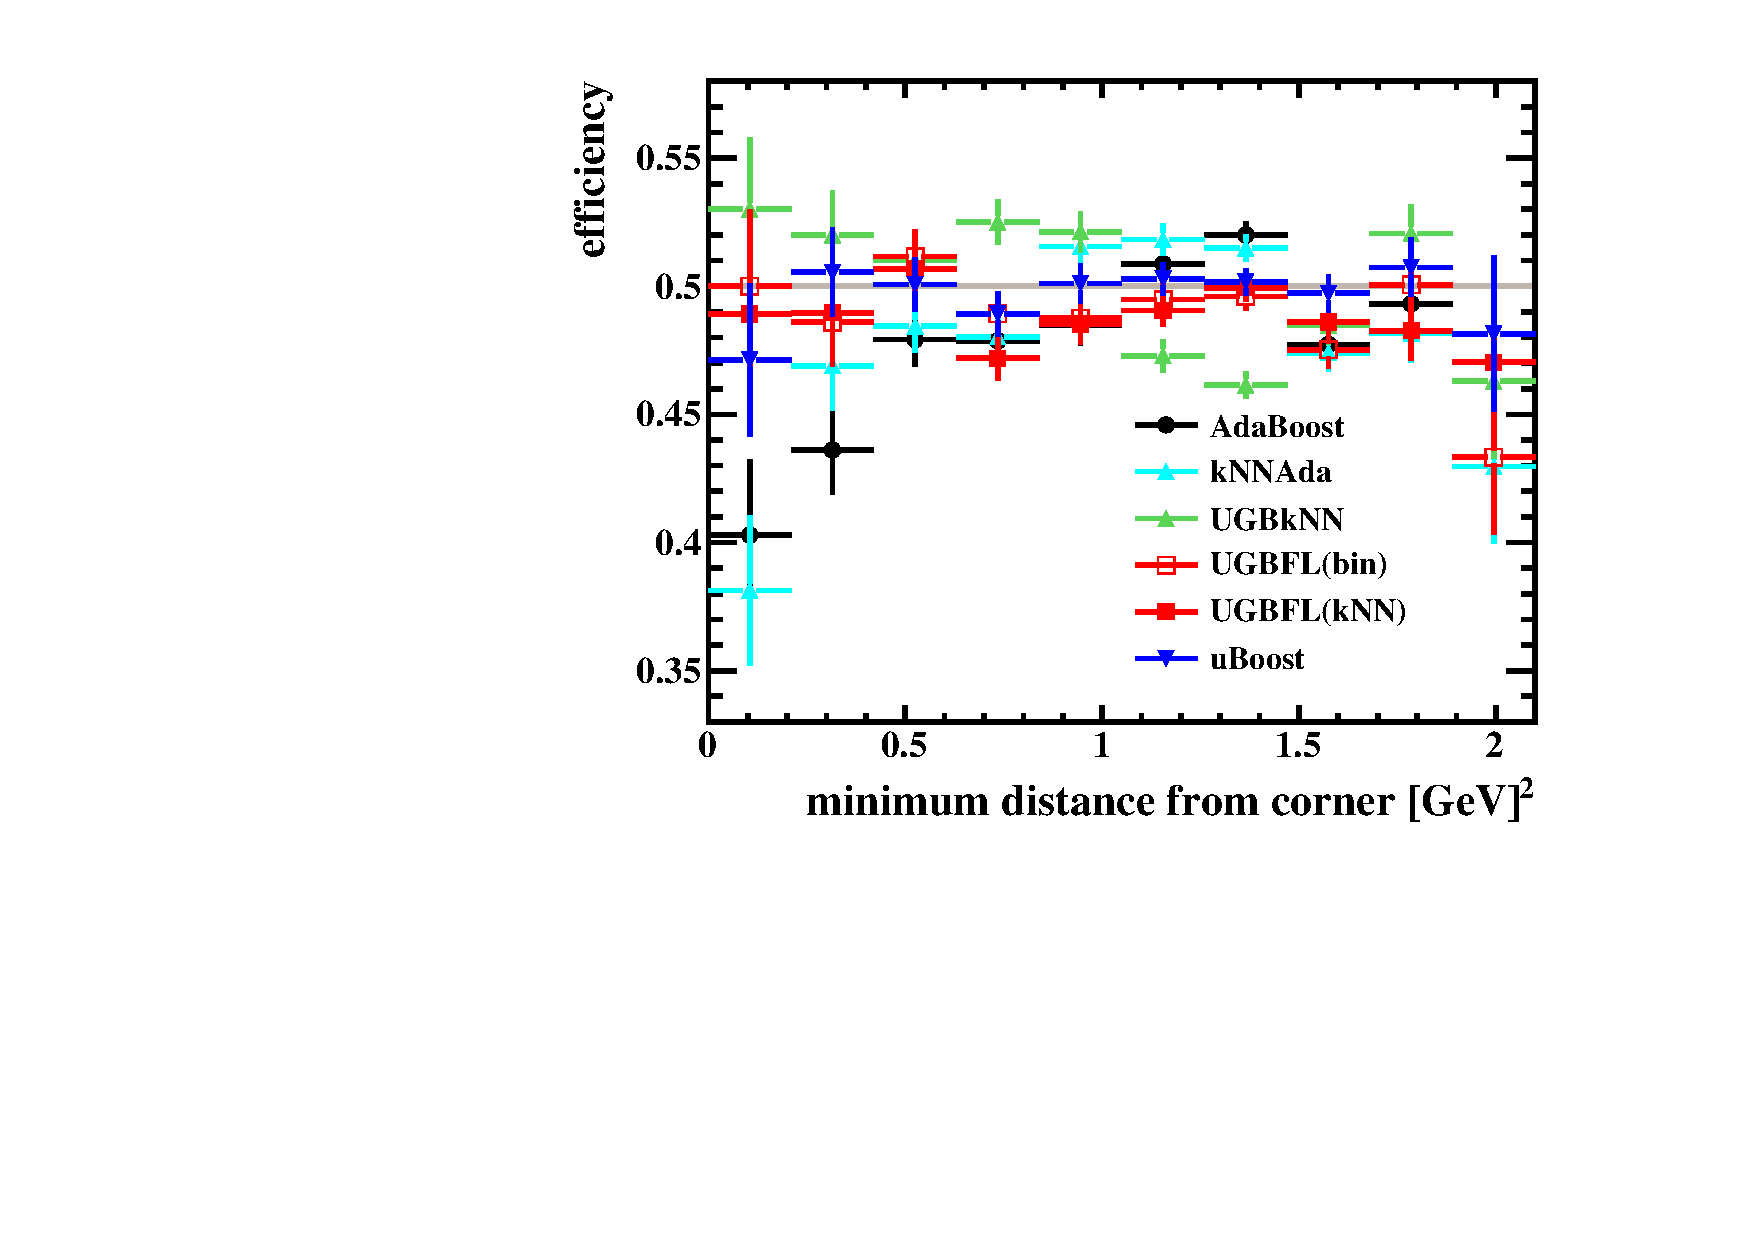
\includegraphics[width=0.49\textwidth]{DP_compare.pdf}
  \caption{\label{fig:dalitz_results} Efficiency {\em vs} distance to a corner of the Dalitz-plot.  An arbitrary working point of 50\% integrated efficiency is displayed.}
\end{figure}

ADD DISCUSSION ON ROC CURVE HERE ...



\begin{figure}[] 
  \centering 
  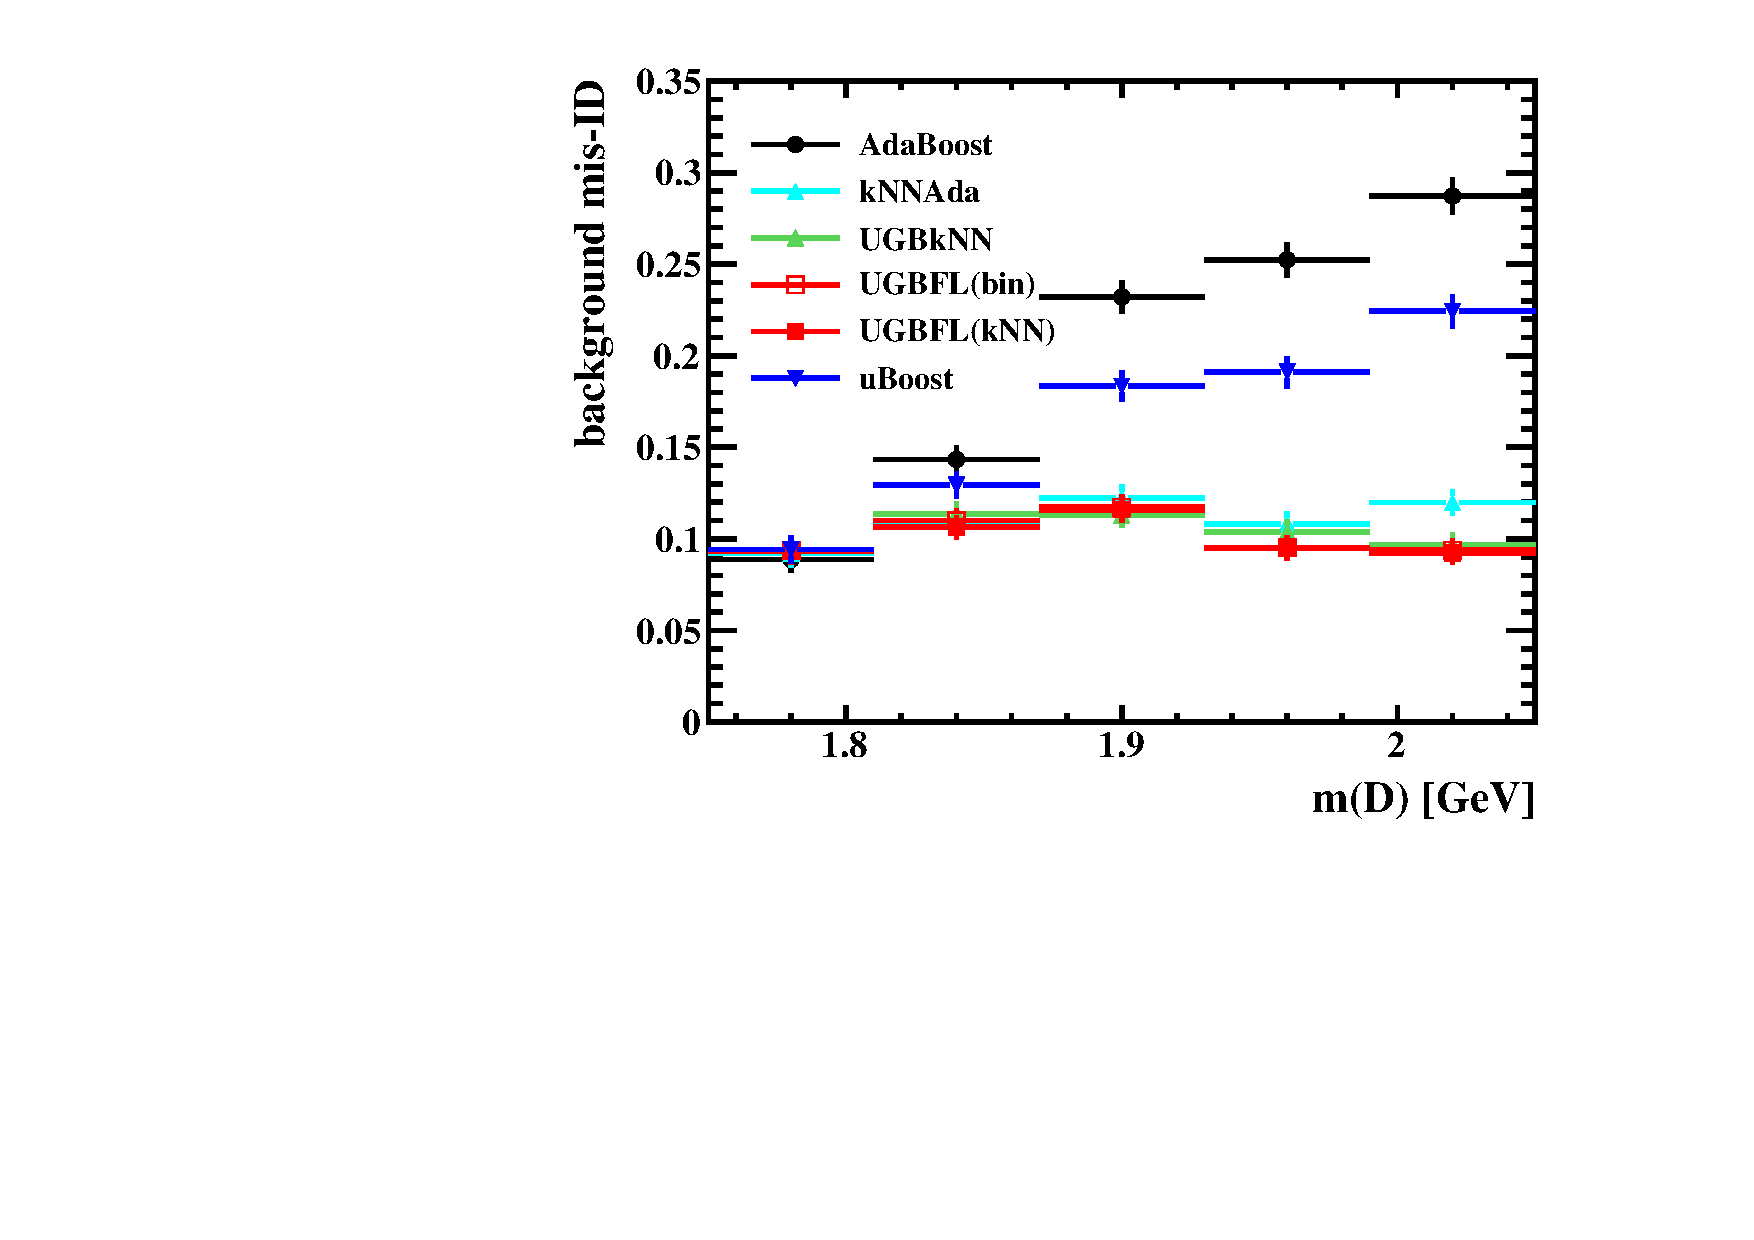
\includegraphics[width=0.49\textwidth]{MD_eff.pdf}
  \caption{\label{fig:dalitz_results} Background mis-identification {\em vs} $D$ candidate mass for (black circles) AdaBoost, (cyan up triangles) kNNAdaBoost, (red filled squares) UGBFL(bin), (red open squares) UGBFL(knn), and (blue down triangles) uBoost.  An arbitrary working point of 10\% background mis-identification in the training region $1.75 < m(D) < 1.85$~GeV is displayed.}
\end{figure}
